\documentclass[11pt]{article}
\usepackage{graphicx}

\begin{document}
	\begin{figure}
		\centering
		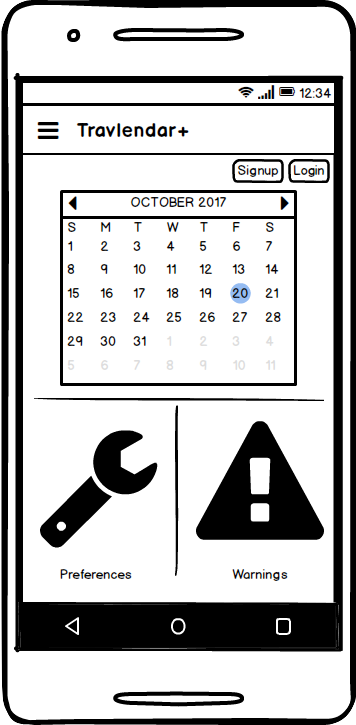
\includegraphics[width=0.7\linewidth]{Homepage.png}
		\caption{This is the homepage of our application.}
		\label{fig:homepage}
	\end{figure}

	\begin{figure}
	\centering
	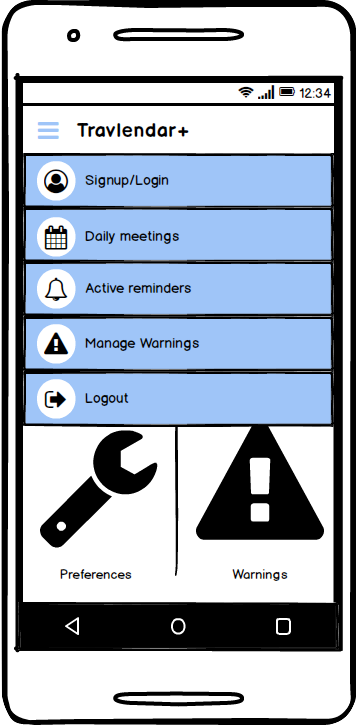
\includegraphics[width=0.7\linewidth]{QuickMenu.png}
	\caption{insert a caption}
	\label{fig:quickmenu}
	\end{figure}

	\begin{figure}
		\centering
		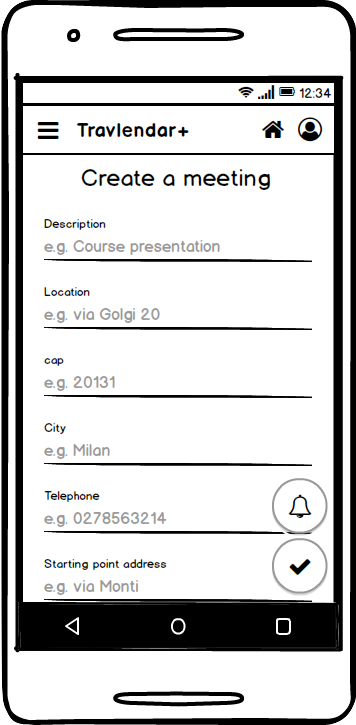
\includegraphics[width=0.7\linewidth]{CreateMeeting.png}
		\caption{the page which allows you to create a meeting}
		\label{fig:createmeeting}
	\end{figure}

	\begin{figure}
	\centering
	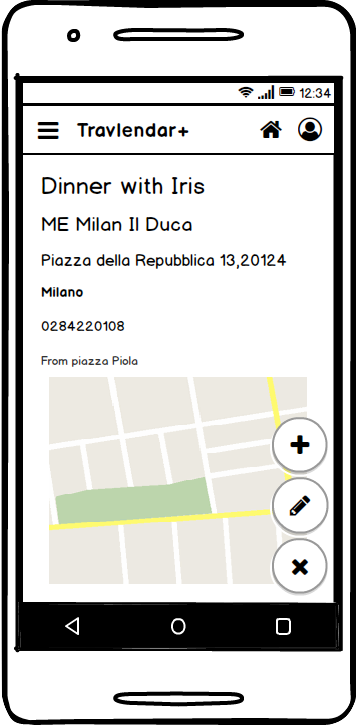
\includegraphics[width=0.7\linewidth]{MeetingView.png}
	\caption{the screen of a meeting page}
	\label{fig:meeting-view}
	\end{figure}

	\begin{figure}
		\centering
		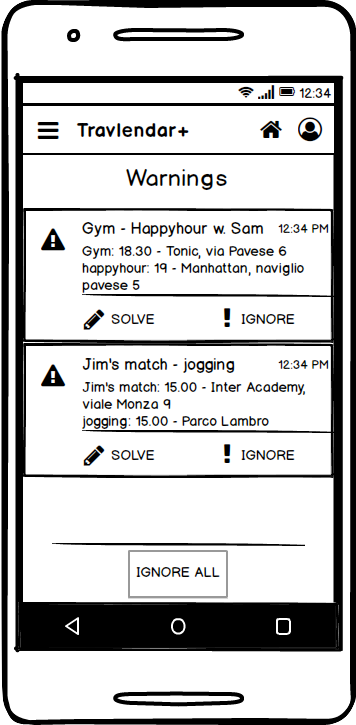
\includegraphics[width=0.7\linewidth]{Warnings.png}
		\caption{insert a caption}
		\label{fig:warnings}
	\end{figure}

		\begin{figure}
		\centering
		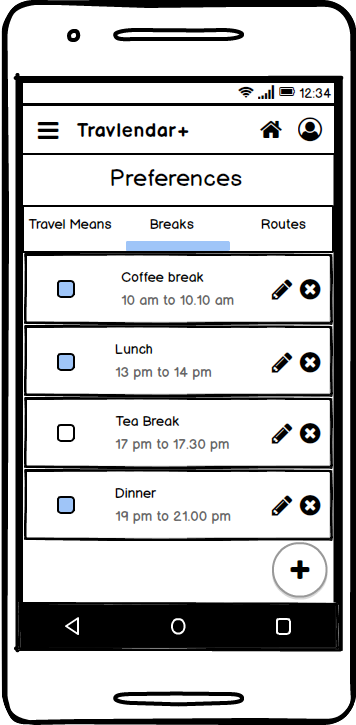
\includegraphics[width=0.7\linewidth]{PreferencesBreaks.png}
		\caption{the page where you can set up your daily breaks}
		\label{fig:preferencesbreaks}
	\end{figure}
	
		\begin{figure}
		\centering
		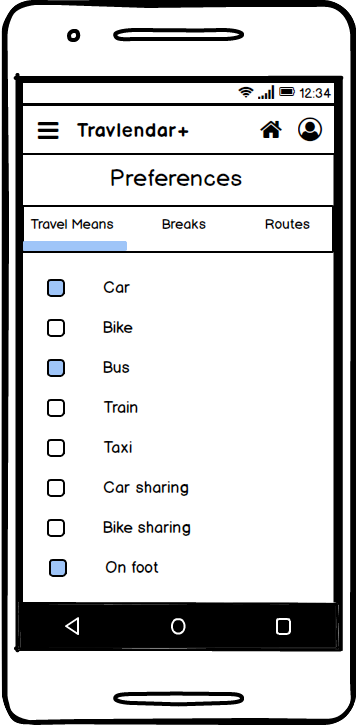
\includegraphics[width=0.7\linewidth]{PreferencesTravelMeans.png}
		\caption{the page where you can select which are the allowed means to reach your meetings}
		\label{fig:preferencestravelmeans}
	\end{figure}
	
		\begin{figure}
		\centering
		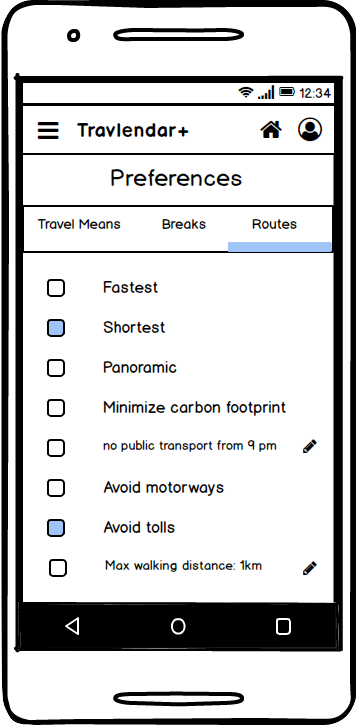
\includegraphics[width=0.7\linewidth]{PreferencesRoutes.png}
		\caption{insert a caption}
		\label{fig:preferencesroutes}
	\end{figure}
	
	


	
\end{document}